\documentclass[12pt]{article}
\usepackage[a4paper,margin=0.75in]{geometry}
\usepackage[utf8]{inputenc}
\usepackage[OT1]{fontenc}
\usepackage[table,usenames,dvipsnames]{xcolor}
\usepackage{array}
\usepackage{varwidth}
\usepackage{tabularx}
\usepackage{hyperref}
\usepackage{enumitem}
\usepackage{graphicx}
\usepackage{tcolorbox}
\renewcommand*\familydefault{\sfdefault}

\newtcolorbox{mybox}[3][]
{
  colframe = #2!25,
  colback  = #2!10,
  coltitle = #2!20!black,  
  title    = {#3},
  #1,
}

\hypersetup{
    colorlinks=true,
    linkcolor=blue,
    filecolor=magenta,      
    urlcolor=cyan,
    pdftitle={Overleaf Example},
    pdfpagemode=FullScreen,
}

\title{\textbf{COL774 Assignment 1}}
\author{Aniruddha Deb \\ \texttt{2020CS10869}}
\date{September 2022}

\begin{document}

\maketitle

\section*{Linear Regression}

\begin{enumerate}[label=(\alph*)]
    \item The parameters we used were:
    \begin{itemize}
        \item Learning rate $\eta = 0.01$
        \item Convergence limit $\epsilon = 0.0001$
        \item Final set of parameters: $(\theta_0,\theta_1) = (0.00561383,0.6451277)$
    \end{itemize}

    \item \raisebox{-.9\height}{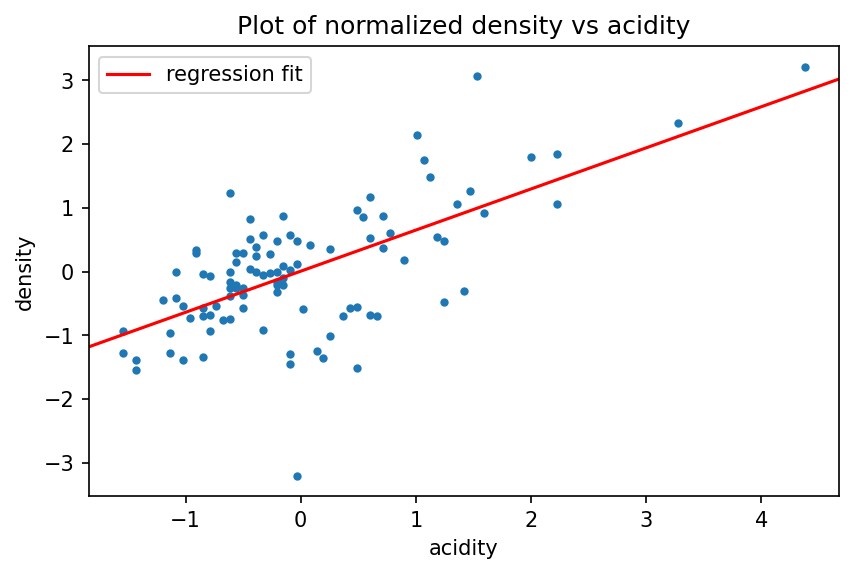
\includegraphics[width=0.7\textwidth]{../Q1/plots/b_plot.png}}

    \item \raisebox{-.9\height}{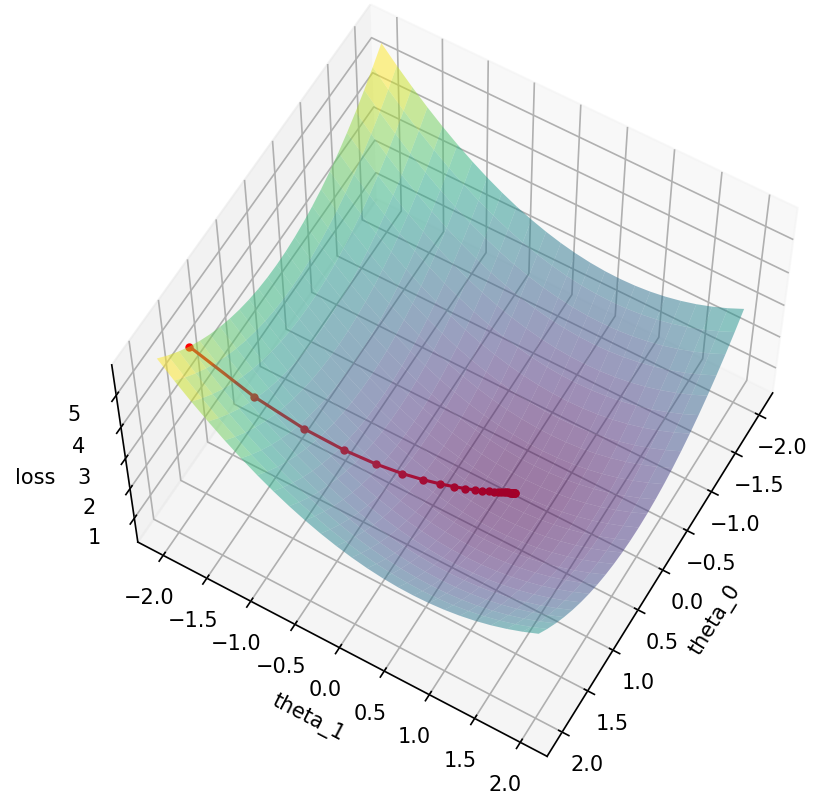
\includegraphics[width=0.7\textwidth]{../Q1/plots/c_mesh.png}}

    \item \raisebox{-.9\height}{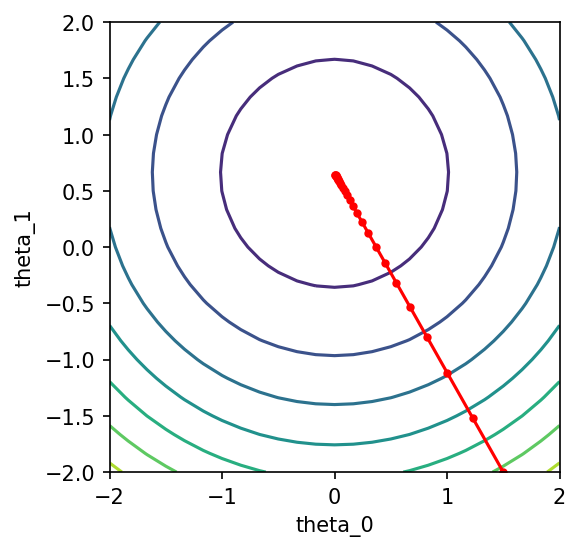
\includegraphics[width=0.7\textwidth]{../Q1/plots/d_contour.png}}

    \item
    \begin{tabular}{c c c}
        $\eta = 0.001$ & $\eta = 0.025$ & $\eta = 0.1$ \\
        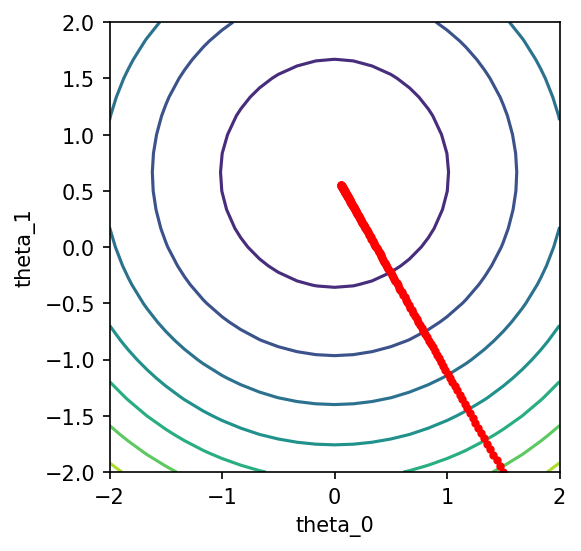
\includegraphics[width=0.3\textwidth]{../Q1/plots/e_contour_001.png} &
        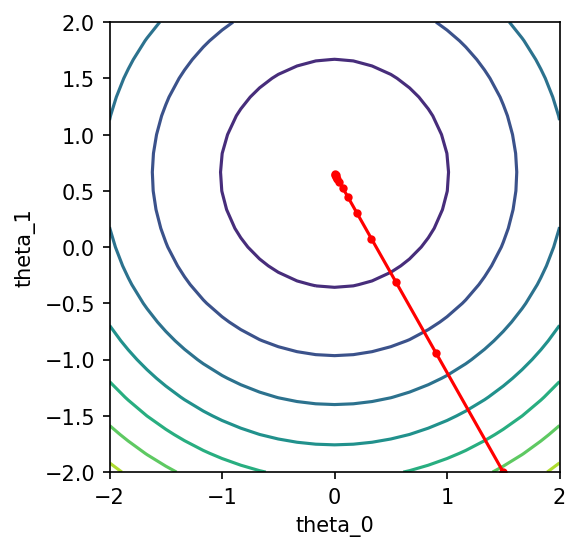
\includegraphics[width=0.3\textwidth]{../Q1/plots/e_contour_025.png} &
        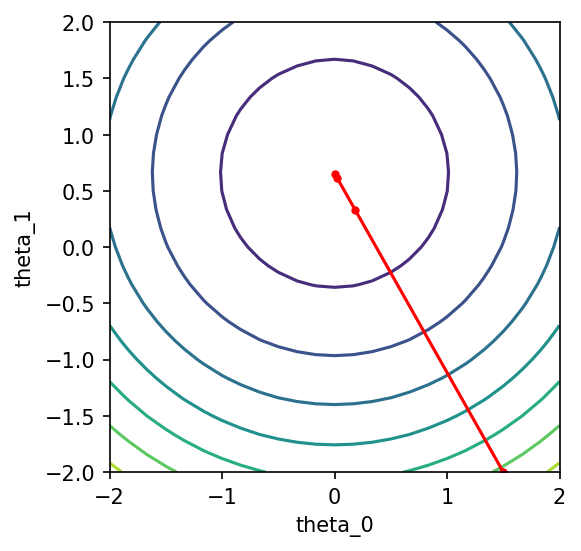
\includegraphics[width=0.3\textwidth]{../Q1/plots/e_contour_1.png} \\
    \end{tabular}

    We notice that with a smaller step size, fewer steps are required to reach convergence; this is beneficial in this case, but can also lead to gradient descent overshooting/not converging in some cases.

\end{enumerate}

\clearpage

\section*{Stochastic Gradient Descent}

\begin{enumerate}
    \addtocounter{enumi}{1}
    \item 
\end{enumerate}

\section*{Logistic Regression}

\section*{Gaussian Discriminant Analysis}

\end{document}
